% \iffalse
\let\negmedspace\undefined
\let\negthickspace\undefined
\documentclass[journal,12pt,twocolumn]{IEEEtran}
\usepackage{cite}
\usepackage{amsmath,amssymb,amsfonts,amsthm}
\usepackage{algorithmic}
\usepackage{graphicx}
\usepackage{textcomp}
\usepackage{xcolor}
\usepackage{txfonts}
\usepackage{listings}
\usepackage{enumitem}
\usepackage{mathtools}
\usepackage{gensymb}
\usepackage{comment}
\usepackage[breaklinks=true]{hyperref}
\usepackage{tkz-euclide} 
\usepackage{listings}
\usepackage{gvv}                                        
\def\inputGnumericTable{}                                 
\usepackage[latin1]{inputenc}                                
\usepackage{color}                                            
\usepackage{array}                                            
\usepackage{longtable}                                       
\usepackage{calc}                                             
\usepackage{multirow}                                         
\usepackage{hhline}                                           
\usepackage{ifthen}                                           
\usepackage{lscape}

\newtheorem{theorem}{Theorem}[section]
\newtheorem{problem}{Problem}
\newtheorem{proposition}{Proposition}[section]
\newtheorem{lemma}{Lemma}[section]
\newtheorem{corollary}[theorem]{Corollary}
\newtheorem{example}{Example}[section]
\newtheorem{definition}[problem]{Definition}
\newcommand{\BEQA}{\begin{eqnarray}}
\newcommand{\EEQA}{\end{eqnarray}}
\newcommand{\define}{\stackrel{\triangle}{=}}
\theoremstyle{remark}
\newtheorem{rem}{Remark}
\begin{document}

\bibliographystyle{IEEEtran}
\vspace{3cm}

\title{NCERT 11.9.5 Q4}
\author{EE23BTECH11038 - Rohith Madhani$^{*}$% <-this % stops a space
}
\maketitle
\newpage
\bigskip
\renewcommand{\thefigure}{\theenumi}
\renewcommand{\thetable}{\theenumi}

\textbf{Question :} Find the sum of all numbers between 200 and 400 which are divisible by 7.\\
\solution 

\begin{table}[!h] 
\centering
\begin{table}[ht]
    \centering
    \begin{tabular}{|c|c|c|}
        \hline
        Parameter & Value & Description \\
        \hline
        $x(0)$ & 5 & First term of AP \\
        $d$ & 1.75 & Common difference of AP \\
        $x(n)$ & 20.75 & $n^{th}$ term of AP \\
        \hline
    \end{tabular}
    \vspace{2mm}
    \caption{Parameter List}
    \label{tab:simple.10.5.2.20}
\end{table}

\caption{Input parameters}
\label{table:11.9.5.4}
\end{table}

The first and last term of the AP are 203 and 399 respectively.
\begin{align}
    \implies x(n) &= (203 + 7n)u(n) 
\end{align}

To calculate the number of terms in the AP,
\begin{align}
    399 &= 203 + 7n \\
    \implies n &= 28
\end{align}

From \eqref{eq:ztrans}
\begin{align}
    X(z) &= \frac{203}{1-z^{-1}} + \frac{7.z^{-1}}{(1-z^{-1})^2} ; |z|>1 \\
    \because y(n) &= x(n)*u(n) \\
    Y(z) &= X(z)U(z) \\
    \implies Y(z) &= \frac{203}{(1-z^{-1})^2} + \frac{7.z^{-1}}{(1-z^{-1})^3} ; |z|>1 
\end{align}

Using Contour integration for inverse Z transform,

\begin{align}
    y(28) &= \frac{1}{2\pi j}\oint_c Y(z) z^{27} dz \\
    &= \frac{1}{2\pi j}\int \frac{203.z^{29}}{(z-1)^{2}} dz + \frac{1}{2\pi j}\int \frac{7.z^{29}}{(z-1)^{3}} dz\\
    \because R&=\frac{1}{\brak {m-1}!}\lim\limits_{z\to a}\frac{d^{m-1}}{dz^{m-1}}\brak {{(z-a)}^{m}f\brak z}\\
    R_1 &=\frac{1}{1!}\lim\limits_{z\to 1}\frac{d}{dz}\brak {(z-1)^2.\frac{203.z^{29}}{(z-1)^{2}}}\\
    &= 203 \times 29 = 5887 \\
    R_2 &=\frac{1}{2!}\lim\limits_{z\to 1}\frac{d^2}{dz^2}\brak {(z-1)^3.\frac{7.z^{29}}{(z-1)^{3}}}\\
    &= \frac{7 \times 29 \times 28}{2!} = 2842\\
    y(28) &= R_1 + R_2 \\
    \implies y(28) &= 8729 
\end{align}

\begin{figure}[h]
  \centering
  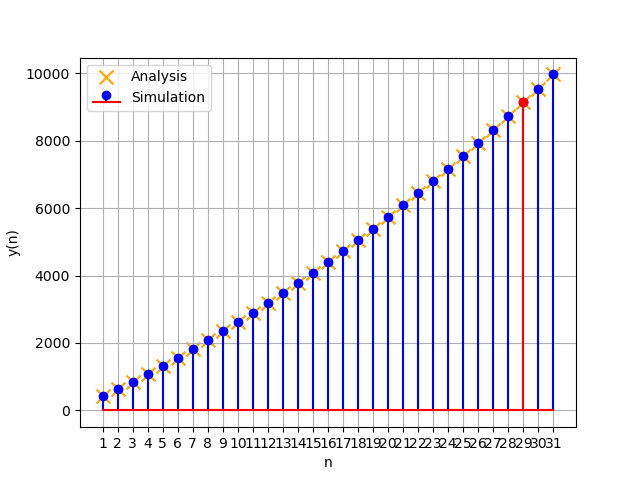
\includegraphics[width=\columnwidth]{figs/fig1.png}
  \caption{y(n) = $199.5n + 3.5n^2$}
  \label{fig:graph}
\end{figure}

\end{document}
